% Fixed data array

\def\inputdata{{
    {2, 3},
    {1, 6}
}}

\def\kerneldata{{
    {5, 2},
    {3, 1}
}}

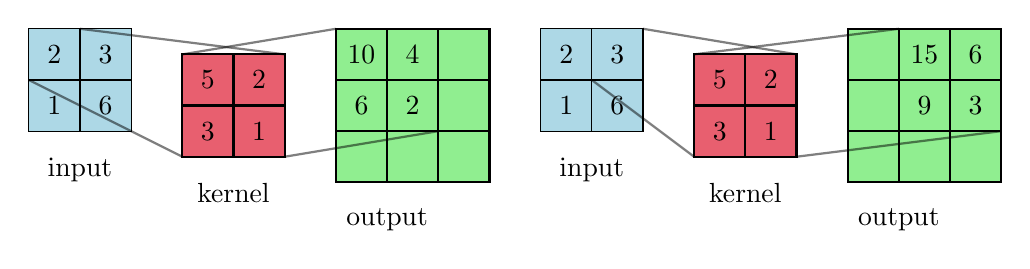
\begin{tikzpicture}[scale=0.65]
\definecolor{inputcolor}{RGB}{173,216,230}
\definecolor{kernelcolor}{RGB}{232,95,111}

% Offsets
\def\xoffset{0}
\def\yoffset{0}

% Draw grid and numbers
\foreach \col in {0,...,1} {
    \foreach \row in {0,...,1} {
        % Get value from array (PGF math arrays are zero-based)
        \pgfmathparse{\inputdata[\row][\col]}
        \let\cellvalue\pgfmathresult

        % Draw at shifted position
        \fill[inputcolor] (\xoffset+\col,\yoffset-\row) rectangle ++(1,-1);
        \draw (\xoffset+\col,\yoffset-\row) rectangle ++(1,-1);

        % Place number centered in shifted position
        \node at (\xoffset+\col+0.5,\yoffset-\row-0.5) {\cellvalue};
    }
}
% Draw kernel grid to the right of input grid
\def\kernelxoffset{3} % Shift right by 3 units (2 for input grid + 1 gap)
\def\kernelyoffset{-0.5}

\foreach \col in {0,...,1} {
    \foreach \row in {0,...,1} {
        \pgfmathparse{\kerneldata[\row][\col]}
        \let\cellvalue\pgfmathresult

        \fill[kernelcolor] (\kernelxoffset+\col,\kernelyoffset-\row) rectangle ++(1,-1);
        \draw[thick,black] (\kernelxoffset+\col,\kernelyoffset-\row) rectangle ++(1,-1);

        \node at (\kernelxoffset+\col+0.5,\kernelyoffset-\row-0.5) {\cellvalue};
    }
}

\draw[opacity=0.5,thick] (1,0) -- (5,-0.5);
\draw[opacity=0.5,thick] (0,-1) -- (3,-2.5);

% Define output grid color
\definecolor{outputcolor}{RGB}{144,238,144}

% Output grid offset (to the right of kernel grid)
\def\outputxoffset{6} % 2 for input + 1 gap + 2 for kernel + 1 gap
\def\outputyoffset{0}

% Output grid values (3x3, only top-left 2x2 filled)
\def\outputdata{{
    {10, 4, ""},
    {6, 2, ""},
    {"", "", ""}
}}

% Draw output grid
\foreach \col in {0,...,2} {
    \foreach \row in {0,...,2} {
        \pgfmathparse{\outputdata[\row][\col]}
        \let\cellvalue\pgfmathresult

        \fill[outputcolor] (\outputxoffset+\col,\outputyoffset-\row) rectangle ++(1,-1);
        \draw[thick,black] (\outputxoffset+\col,\outputyoffset-\row) rectangle ++(1,-1);

        % Only show non-empty values
        \ifx\cellvalue\empty
            % Do nothing
        \else
            \node at (\outputxoffset+\col+0.5,\outputyoffset-\row-0.5) {\cellvalue};
        \fi
    }
}

\draw[opacity=0.5,thick] (6,0) -- (3,-0.5);
\draw[opacity=0.5,thick] (8,-2) -- (5,-2.5);

% Shift for second set of grids
\def\secondshift{10}

% Draw second input grid
\foreach \col in {0,...,1} {
    \foreach \row in {0,...,1} {
        \pgfmathparse{\inputdata[\row][\col]}
        \let\cellvalue\pgfmathresult

        \fill[inputcolor] (\secondshift+\xoffset+\col,\yoffset-\row) rectangle ++(1,-1);
        \draw (\secondshift+\xoffset+\col,\yoffset-\row) rectangle ++(1,-1);

        \node at (\secondshift+\xoffset+\col+0.5,\yoffset-\row-0.5) {\cellvalue};
    }
}

% Draw second kernel grid
\foreach \col in {0,...,1} {
    \foreach \row in {0,...,1} {
        \pgfmathparse{\kerneldata[\row][\col]}
        \let\cellvalue\pgfmathresult

        \fill[kernelcolor] (\secondshift+\kernelxoffset+\col,\kernelyoffset-\row) rectangle ++(1,-1);
        \draw[thick,black] (\secondshift+\kernelxoffset+\col,\kernelyoffset-\row) rectangle ++(1,-1);

        \node at (\secondshift+\kernelxoffset+\col+0.5,\kernelyoffset-\row-0.5) {\cellvalue};
    }
}

\draw[opacity=0.5,thick] (\secondshift+2,0) -- (\secondshift+5,-0.5);
\draw[opacity=0.5,thick] (\secondshift+1,-1) -- (\secondshift+3,-2.5);
% Draw second output grid
% Top right 2x2 subgrid: positions (0,1), (0,2), (1,1), (1,2)
\def\secondoutputdata{{
    {"", 15, 6},
    {"", 9, 3},
    {"", "", ""}
}}

\foreach \col in {0,...,2} {
    \foreach \row in {0,...,2} {
        \pgfmathparse{\secondoutputdata[\row][\col]}
        \let\cellvalue\pgfmathresult

        \fill[outputcolor] (\secondshift+\outputxoffset+\col,\outputyoffset-\row) rectangle ++(1,-1);
        \draw[thick,black] (\secondshift+\outputxoffset+\col,\outputyoffset-\row) rectangle ++(1,-1);

        \ifx\cellvalue\empty
        \else
            \node at (\secondshift+\outputxoffset+\col+0.5,\outputyoffset-\row-0.5) {\cellvalue};
        \fi
    }
}

\draw[opacity=0.5,thick] (\secondshift+7,0) -- (\secondshift+3,-0.5);
\draw[opacity=0.5,thick] (\secondshift+9,-2) -- (\secondshift+5,-2.5);

% Labels for first set
\node[below=6pt] at (1,-2) {input};
\node[below=6pt] at (4,-2.5) {kernel};
\node[below=6pt] at (7,-3) {output};

% Labels for second set
\node[below=6pt] at (\secondshift+1,-2) {input};
\node[below=6pt] at (\secondshift+4,-2.5) {kernel};
\node[below=6pt] at (\secondshift+7,-3) {output};

\end{tikzpicture}